\documentclass{PHKA_inf} 
%add the additional packages and macros that you want to use
%here you can find some useful additional packages and macros

%Package to show algorithms
\usepackage{algorithm2e}

%package to work with glossaries
\usepackage[acronym]{glossaries}

%packages and setings to show colored code
\usepackage{listings}
\usepackage{xcolor}

\definecolor{codegreen}{rgb}{0,0.6,0}
\definecolor{codegray}{rgb}{0.5,0.5,0.5}
\definecolor{codepurple}{rgb}{0.58,0,0.82}
\definecolor{backcolour}{rgb}{0.95,0.95,0.92}

\lstdefinestyle{mystyle}{
    backgroundcolor=\color{backcolour},   
    commentstyle=\color{codegreen},
    keywordstyle=\color{magenta},
    numberstyle=\tiny\color{codegray},
    stringstyle=\color{codepurple},
    basicstyle=\ttfamily\footnotesize,
    breakatwhitespace=false,         
    breaklines=true,                 
    captionpos=b,                    
    keepspaces=true,                 
    numbers=left,                    
    numbersep=5pt,                  
    showspaces=false,                
    showstringspaces=false,
    showtabs=false,                  
    tabsize=2
}

\lstset{style=mystyle}

%package to allow comments/notes by you and other people
\usepackage[multiuser,marginclue,nomargin,inline,index]{fixme}
\definecolor{ttwgreen}{RGB}{75,135,73}
\fxusetheme{colorsig}
%\FXRegisterAuthor{tm}{atm}{\color{red}TM}
\FXRegisterAuthor{ttw}{attw}{\color{ttwgreen}TTW} % creates ttwnote, ttwwarning, ttwerror, ttwfatal commands
%\FXRegisterAuthor{mk}{amk}{\color{blue}MK}

%add your own packages or macros here
\usepackage[round]{natbib} 
% important update for glossaries, before document 
\loadglsentries{C) Back Matter/acronyms.tex}
\loadglsentries{C) Back Matter/glossary.tex} 
% \makeglossaries %https://www.overleaf.com/learn/latex/glossaries

%shows fixme notes
%\fxsetup{status=draft} % comment/delete this line if you want to your final output

\usepackage[ngerman]{babel} %if changed to \usepackage[ngerman]{babel} "Table of contents" changes to "Inhaltsverzeichnis", "abstract" becomes "Zusammenfassung" and "references" is translated to "Literatur".
\usepackage{makecell}
\usepackage{float}
\usepackage{longtable}
\usepackage{hyperref}
\hypersetup{
  colorlinks=true,
  linkcolor=black,
  urlcolor=blue!70!black
}


%remove all the things you don't need and add all the things you need. you can also change the order of the elements at your will.
\begin{document}

    %Start with front matter
    \Titlepage
 %Creates the titlepage


    

% 	\frontmatter{}
	
	\cleardoublepage{}
	
	\cleardoublepage{}


	
    \microtypesetup{protrusion=false}
    \tableofcontents{}
    \listoftables
    % Use an optional list of tables / figures / algorithms / listings(code).
 
    \cleardoublepage{}
    
    
    \cleardoublepage{}
   
    \cleardoublepage{}
    \microtypesetup{protrusion=true}
    

	
	
	\mainmatter{}
	%add your chapters here
	%Comment Chapters with "%" to exclude them
	
	%Kapitel
    \chapter{Einleitung}

\section{Thema und Motivation}
Das Iterative Gefangenendilemma (IPD) ist ein klassisches Problem der Spieltheorie, 
das die Herausforderungen von Kooperation und Eigennutz modelliert. 
Zwei Spieler müssen unabhängig voneinander entscheiden, ob sie kooperieren oder 
defektieren. Während Kooperation zu einem besseren kollektiven Ergebnis führt, 
ist aus individueller Sicht Defektion oft vorteilhafter – ein klassisches Dilemma.
In der Realität tauchen ähnliche Dilemmata in vielen Bereichen auf, etwa in der 
Wirtschaft, der Politik und der Evolutionsbiologie. Ein zentrales Forschungsthema 
ist, ob und unter welchen Bedingungen Akteure langfristig kooperative Strategien 
entwickeln können, um dem Dilemma zu entkommen.

Mit der zunehmenden Bedeutung von künstlicher Intelligenz (KI) und Reinforcement 
Learning (RL) stellt sich die Frage, wie sich autonome Agenten in einem solchen 
Szenario verhalten. Können sie durch Lernen langfristig Kooperation aufbauen, 
oder werden sie egoistische Strategien bevorzugen? Ziel dieses Projekts ist es, 
RL-Agenten im IPD zu trainieren und zu analysieren, ob sie fähig sind, Strategien 
zu entwickeln, die über bloßen Eigennutz hinausgehen. Damit trägt diese Arbeit zur 
Diskussion über das Potenzial von RL in sozialen und spieltheoretischen Kontexten 
bei.

\section{Ziele der Arbeit}
Das Ziel dieser Arbeit ist es, zu untersuchen, wie sich RL-Agenten im IPD verhalten
und ob sie in der Lage sind, kooperative Strategien zu entwickeln. Dabei stehen 
folgende zentrale Forschungsfragen im Fokus:
\begin{enumerate}
    \item Können RL-Agenten lernen, langfristig zu kooperieren?
        \begin{itemize}
            \item Entwickeln sie Strategien, die über reines Eigeninteresse hinausgehen?
            % \item Gibt es bestimmte Bedingungen, unter denen Kooperation wahrscheinlicher wird?
        \end{itemize}
    \item Welche Strategien entstehen im Laufe des Lernprozesses?
        \begin{itemize}
            \item Verhalten sich die Agenten wie bekannte spieltheoretische Strategien (z. B. ''Tit-for-Tat'' oder ''Always Defect'')?
            \item Zeigen sich neuartige, unerwartete Verhaltensmuster?
        \end{itemize}
    % \item Wie beeinflussen verschiedene Lernparameter das Verhalten der Agenten?
    %     \begin{itemize}
    %         \item Welche Rolle spielen Faktoren wie Belohnungsfunktionen, Discount-Faktor oder Explorationsstrategien?
    %         \item Wie wirken sich unterschiedliche Trainingsumgebungen auf die Ergebnisse aus?
    %     \end{itemize}
\end{enumerate}
Um diese Fragen zu beantworten, werden verschiedene RL-Algorithmen auf das IPD 
angewendet, die Trainingsverläufe analysiert und die resultierenden Strategien 
miteinander verglichen. Durch die gewonnenen Erkenntnisse soll ein tieferes Verständnis 
dafür geschaffen werden, wie lernende Agenten spieltheoretische Herausforderungen 
bewältigen und ob sie sich aus dem klassischen Dilemma befreien können.
    \chapter{Hintergrund und theoretischer Rahmen}
\section{Das Iterierter Gefangenendilemma}
Das Gefangenendilemma ist eines der bekanntesten Probleme der Spieltheorie und 
beschreibt eine Situation, in der zwei Spieler unabhängig voneinander entscheiden 
müssen, ob sie kooperieren oder defektieren. Die Auszahlung für jeden Spieler hängt 
sowohl von der eigenen Entscheidung als auch von der des Gegenübers ab. 
Die klassische Auszahlungsmatrix sieht dabei folgendermaßen aus:

\begin{table}[h!]
    \centering
    \begin{tabular}{c|c|c}
            & Spieler B kooperiert & Spieler B defektiert\\
        \hline
        Spieler A kooperiert &  \makecell{(R, R) \\ Belohnung für Kooperation} & \makecell{(S, T) \\ A verliert, B gewinnt} \\
        \hline
        Spieler A defektiert &  \makecell{(T, S) \\ A gewinnt, B verliert} & \makecell{(P, P) \\ Bestrafung für gegenseitige Defektion} \\
    \end{tabular}
    \caption{Allgemeine Auszahlungsmatrix}
    \label{table:allgemeineauszahlungsmatrix}
\end{table}

Dabei gilt üblicherweise:
\begin{itemize}
    \item T (Temptation) > R (Reward) > P (Punishment) > S (Sucker's payoff)
    \item 2R > T + S, sodass sich gegenseitige Kooperation langfristig mehr lohnen würde als wechselseitige Ausnutzung.
\end{itemize}
Im einmaligen Gefangenendilemma ist die dominante Strategie, zu defektieren, da 
dies in jedem individuellen Fall die höhere Auszahlung sichert – unabhängig von der 
Entscheidung des Gegenspielers. Dies führt jedoch zu einem sozial suboptimalen 
Ergebnis.

Im iterierten Gefangenendilemma (IDG) wird das Spiel jedoch mehrfach hintereinander 
gespielt, sodass frühere Entscheidungen zukünftige Interaktionen beeinflussen können. 
Dadurch eröffnen sich neue Möglichkeiten für kooperative Strategien, bei denen 
Agenten versuchen, durch wechselseitige Zusammenarbeit langfristig höhere Erträge 
zu erzielen. Bekannte Strategien aus der Spieltheorie für das IDG sind beispielsweise:
"Tit-for-Tat" (Spiele das, was dein Gegner in der vorherigen Runde getan hat).
"Always Defect" (Immer defektieren, um kurzfristig die höchste Auszahlung zu sichern).
"Grim Trigger" (Kooperiere, aber falls der Gegner einmal defektiert, defektiere für immer).

Die zentrale Forschungsfrage im IPD lautet daher: Ist es möglich, langfristige 
Kooperation zu etablieren, oder führt Eigennutz immer zu gegenseitiger Defektion? 
Diese Fragestellung ist besonders relevant für Reinforcement Learning-Agenten, da 
sie ihre Strategie durch wiederholte Interaktion und Belohnungsmechanismen erlernen.

\section{Reinforcement Learning}
Reinforcement Learning (RL) ist ein Teilbereich des maschinellen Lernens, bei dem 
ein Agent durch Interaktion mit einer Umgebung eine optimale Strategie erlernt. 
Der Lernprozess basiert auf einem Belohnungssystem: Der Agent führt Aktionen aus, 
erhält daraufhin Belohnungen oder Bestrafungen und passt sein Verhalten 
entsprechend an. RL-Probleme werden typischerweise als Markov-Entscheidungsprozesse 
(MDP) modelliert, bestehend aus:
\begin{itemize}
    \item Zustand (State, $S$): Die aktuelle Situation der Umgebung.
    \item Aktion (Action, $A$): Eine Entscheidung, die der Agent treffen kann.
    \item Belohnung (Reward, $R$): Eine Rückmeldung, die die Qualitaten der gewählten Aktion bewertet.
    \item Übergangsmodell ($P(s' \vert s, a)$): Wahrscheinlichkeiten, dass der Zustand $s'$ nach einer Aktion $a$ im Zustand $s$ entsteht.
    \item Policy ($\pi(s)$): Die Strategie des Agenten zur Auswahl von Aktionen.
\end{itemize}
Das Ziel ist es, eine Optimale Policy $\pi^*$ zu lernen, die die kumulierte zukünftige Belohnung maximiert. 
Dafür gibt es verschiedene Methoden, darunter Q-Learning und Deep Q-Learning.

\subsection{Q-Learning}
Q-Learning ist ein wertbasierter RL-Algorithmus, der darauf abzielt, die Q-Werte 
für jede Zustands-Aktions-Kombination zu erlernen. Der Q-Wert $Q(s,a)$ repräsentiert 
die erwartete zukünftige Belohnung, wenn der Agent in Zustand $s$ Aktion $a$ wählt 
und danach der optimalen Strategie folgt.
Die Aktualisierung der Q-Werte erfolgt iterativ mit der Bellman-Gleichung:
\begin{equation}
    Q(s,a) \leftarrow Q(s,a) + \alpha (r + \gamma \max_{a'}Q(s',a') - Q(s,a))
\end{equation}
Hierbei sind:
\begin{itemize}
    \item $\alpha$ die Lernrate, die bestimmt, wie stark neue Informationen alte Werte überschreiben.
    \item $\gamma$ der Diskontfaktor, der die Gewichtung zukünftiger Belohnungen bestimmt.
    \item $r$ die unmittelbare Belohnung nach der Aktion $a$.
\end{itemize}
Da Q-Learning tabellarisch arbeitet, ist es nur für kleine Zustandsräume geeignet, 
da die Q-Tabelle bei vielen möglichen Zuständen und Aktionen schnell zu groß wird. 
In komplexeren Umgebungen ist daher eine neuronale Netzarchitektur notwendig - 
hier kommt Deep Q-Learning (DQN) ins Spiel.

\subsection{Deep Q-Learning}
Deep Q-Learning (DQN) erweitert Q-Learning durch den Einsatz eines neuronalen 
Netzwerks zur Approximation der Q-Werte, anstatt eine explizite Tabelle zu 
speichern. Dies erlaubt das Lernen in hochdimensionalen Zustandsräumen, die 
tabellarische Methoden überfordern würden.
Die Hauptbestandteile von DQN sind:
\begin{enumerate}
    \item Neuronales Netz als Q-Funktion
        \begin{itemize}
            \item Das Netz nimmt den Zustand $s$ als Eingabe und gibt geschätzte Q-Werte für alle möglichen Aktionen $a$ aus.
            \item Die Gewichte des Netzwerks werden durch Gradientenabstieg und einen Mean-Squared-Error (MSE)-Loss aktualisiert.
        \end{itemize}
    \item Erfahrungsspeicher (Experience Replay)
        \begin{itemize}
            \item Anstatt direkt mit den neuesten Erfahrungen zu trainieren, werden vergangene Erfahrungen $(s,a,r,s')$ in einem Speicher abgelegt.
        \end{itemize}
    \item Zielnetzwerk (Target Network)
        \begin{itemize}
            \item Zusätzlich zum Hauptnetzwerk existiert eine separate Kopie, die in regelmäßigen Abständen aktualisiert wird.
            \item Dies verhindert zu starke Schwankungen in den Q-Werten und stabilisiert das Training.
        \end{itemize}
\end{enumerate}
Die Aktualisierungsregel für DQN basiert auf dem Mean-Squared-Error zwischen dem 
vorhergesagten und dem Ziel-Q-Wert:
\begin{equation}
    L = \left(r + \gamma \max_{\alpha'}Q_{\text{target}}(s',a') - Q_{\text{current}}(s,a)\right)^2
\end{equation}
DQN ist besonders mächtig für komplexe Umgebungen, in denen eine tabellarische 
Q-Funktion nicht mehr praktikabel ist.

% \section{Verwandte Arbeiten}
    \chapter{Methodik}
\section{Aufbau des Experiments}
Um zu untersuchen, wie Reinforcement-Learning-Agenten im Iterierten 
Gefangenendilemma (IPD) agieren, wurde eine experimentelle 
\href{https://github.com/Jonah-gr/Reinforcement-Learning-IPD}{Python-Umgebung} implementiert. 
Diese Umgebung ermöglicht es, Spiele zu simulieren, RL-Agenten zu trainieren, und diese dann zu evaluieren.
Für all diese Zwecke wurde die Rundenanzahl pro Spiel auf $n=100$ gesetzt und die folgende Auszahlungsmatrix verwendet:

\begin{table}[h!]
    \centering
    \begin{tabular}{c|c|c}
            & Spieler B kooperiert & Spieler B defektiert\\
        \hline
        Spieler A kooperiert &  (3, 3) & (5, 0) \\
        \hline
        Spieler A defektiert &  (0, 5) & (1, 1) \\
    \end{tabular}
    \caption{Auszahlungsmatrix}
    \label{table:auszahlungsmatrix}
\end{table}

\section{Agenten und Strategien}
Für das Training und die Evaluation der RL-Agent wurden folgende Basis-Strategien implementiert:

\begin{longtable}{|c|m{7cm}|}
    \hline
    \textbf{Strategie} & \textbf{Beschreibung} \\
    \hline
    RandomAgent() & Entscheidet zufällig \\
    \hline
    AlwaysCooperateAgent() & Kooperiert immer \\
    \hline
    AlwaysDefectAgent() & Verrät immer \\
    \hline
    ProvocativeAgent() & Verrät nach zweimaligem Kooperieren \\
    \hline
    TitForTatAgent() & Imitiert den Gegner \\
    \hline
    TitForTwoTatsAgent() & Verrät, wenn der Gegner zweimal verrät \\
    \hline
    TwoTitsForTatAgent() & Verrät zweimal, wenn der Gegner verrät \\
    \hline
    TitForTatOppositeAgent() & Imitiert den Gegner umgekehrt \\
    \hline
    SpitefulAgent() & Verrät immer, wenn der Gegner verrät \\
    \hline
    GenerousTitForTatAgent() & Imitiert den Gegner, vergibt aber in 10\% der Fälle \\
    \hline
    AdaptiveAgent() & Verrät, wenn der Gegner in den letzten 10 Runden zu mehr als 50\% verraten hat \\
    \hline
    PavlovAgent() & Verrät, wenn die Entscheidungen in der vorherigen Runde unterschiedlich waren \\
    \hline
    GradualAgent() & Verrät so oft, wie der Gegner verrät \\
    \hline
    WinStayLoseShiftAgent() & Ändert die Strategie, wenn die letzte Belohnung < 1 war \\
    \hline
    SoftMajorityAgent() & Verrät, wenn der Gegner in mehr als 50\% der Fälle verrät \\
    \hline
    SuspiciousTitForTatAgent() & Imitiert den Gegner und verrät in der ersten Runde \\
    \hline
    SuspiciousAdaptiveAgent() & Verrät, wenn der Gegner in den letzten 10 Runden zu mehr als 50\% verraten hat, und verrät in der ersten Runde \\
    \hline
    SuspiciousGenerousTitForTatAgent() & Imitiert den Gegner, vergibt aber in 10\% der Fälle und verrät in der ersten Runde \\
    \hline
    SuspiciousGradualAgent() & Verrät so oft, wie der Gegner verrät, und verrät in der ersten Runde \\
    \hline
    SuspiciousPavlovAgent() & Verrät, wenn die Entscheidungen in der vorherigen Runde unterschiedlich waren, und verrät in der ersten Runde \\
    \hline
    SuspiciousSoftMajorityAgent() & Verrät, wenn der Gegner in mehr als 50\% der Fälle verrät, und verrät in der ersten Runde \\
    \hline
    SuspiciousTitForTwoTatsAgent() & Verrät, wenn der Gegner zweimal verrät, und verrät in der ersten Runde \\
    \hline
    SuspiciousTwoTitsForTatAgent() & Verrät zweimal, wenn der Gegner verrät, und verrät in der ersten Runde \\
    \hline
    SuspiciousWinStayLoseShiftAgent() & Ändert die Strategie, wenn die letzte Belohnung < 1 war, und verrät in der ersten Runde \\
    \hline
\caption{Basis-Strategien}
\label{table:basestrategies}
\end{longtable}

Der Q-Learning Agent nutzt eine Q-Tabelle zur Approximation der Q-Werte.
Hierbei steuert die Lernrate $\alpha=0.001$, wie stark neue Informationen in die Q-Tabelle einfließen, während der 
Discount-Faktor $\gamma=0.95$ zukünftige Belohnungen mit einbezieht. Der Agent nutzt eine $\epsilon$-greedy Strategie, 
bei der mit Wahrscheinlichkeit $\epsilon$ eine zufällige Aktion gewählt wird, um Exploration zu ermöglichen. 
$\epsilon$ startet bei 1.0 und wird mit 0.9995 pro Runde reduziert, bis ein Minimum von 0.00001 erreicht ist. 
Zur Entscheidungsfindung nutzt er entweder zufällige
Exploration oder wählt die Aktion mit dem höchsten Q-Wert basierend auf der letzten Gegneraktion. \\

Der Deep Q-Learning Agent nutzt ein neuronales Netzwerk zur Approximation der Q-Werte und basiert auf einem 
Feedforward-Netzwerk mit drei voll verbundenen Schichten: Eine Eingabeschicht mit 64 Neuronen, eine versteckte 
Schicht mit 32 Neuronen und eine Ausgabeschicht mit 2 Neuronen, die die Q-Werte für die beiden möglichen Aktionen 
(Kooperation oder Defektion) liefert. ReLU-Aktivierungen sorgen für nicht-lineare Modellierung, während Xavier-Initialisierung 
eine stabile Gewichtsverteilung gewährleistet. Diese sorgt dafür, dass die Gewichte so initialisiert werden, dass der 
Informationsfluss durch das Netzwerk stabil bleibt. Die Gewichte $W$ werden so initialisiert, dass
\begin{equation}
    W \sim U \left( -\frac{\sqrt{6}}{\sqrt{n_{\text{in}}+n_{\text{out}}}}, \frac{6}{\sqrt{n_{\text{in}}+n_{\text{out}}}} \right)
\end{equation}
mit $n_{in}$ und $n_{out}$ als Anzahl der Neuronen der vorherigen und der aktuellen Schicht. Die Varianz der Gewichte bleibt
also über alle Schichten hinweg konstant.
Das Netz bekommt die letzten zehn Runden, also einen 20-dimensionalen 
Zustandsvektor, als Eingabe. Der Agent nutzt eine Replay-Memory (max. 20.000 Einträge) zur stabileren 
Lernprozessgestaltung und ein $\epsilon$-greedy Explorationsverfahren, bei dem die Wahrscheinlichkeit für zufällige Aktionen mit 
zunehmendem Training abnimmt ($\epsilon$ sinkt von 1.0 auf 0.00001 mit einem Faktor von 0.9995). Das Lernen erfolgt über MSE-Loss und Adam-Optimierung mit 
einer Lernrate von 0.001.
Während des Trainings werden zufällige 5 Batches aus der Replay-Memory gezogen und die Q-Werte 
aktualisiert, wobei der jeweilige optimale Q-Wert (Ausgabe des Zielnetzwerks) mit $\gamma=0.95$ diskontiert wird.

Die Belohnunsfunktion beider RL-Agenten ist die vorher beschriebene Auszahlungsmatrix (siehe Tab. \ref{table:auszahlungsmatrix}). \\ \\
Beide RL-Agenten wurden in 10000 Episoden gegen eine zufällige aber feste Reihenfolge von Basis-Agenten trainiert.


\section{Evaluierungsmethodik}
Die Evaluierungsmethodik basiert auf einem Turnierformat, in dem jeder Agent gegen jeden Basis-Agenten 100 Spiele 
absolvieren muss. Jeder Agent spielt also $24 * 100 = 2400$ Spiele (es gibt 24 Basis-Agenten) und $2400 * 100 = 240000$ Runden. Dieses Format
stellt sicher, dass für alle Agenten die selben Voraussetzungen herrschen und statistisch signifante Ergebnisse erzielt werden.

    \chapter{Ergebnisse}
\section{Daten und Beobachtungen}
Über die $T = 10000$ Trainingsepisoden wurden folgende durchschnittliche Belohnungen pro Epsiode berechnet:
\begin{table}[H]
    \centering
    \begin{tabular}{c|c}
            & $\frac{\sum r}{T}$ \\
        \hline
        QLearningAgent($\alpha$ = 0.1, $\gamma$ = 0.95)  & 265 \\
        \hline
        DeepQLearningAgent($\alpha$ = 0.001, $\gamma$ = 0.95) & 287 \\
        \hline
        RandomStrategies() & 233
    \end{tabular}
    \caption{Trainigs-Ergebnisse}
    \label{table:trainingsergebnisse}
\end{table}
Es bildet sich also schon während des Trainings ab, dass der QLearning-Agent und der Deep QLearning-Agent langfristig
bessere Entscheidungen treffen, als der \textit{RandomStrategies()} Agent. Es lohnt sich also weniger jedes Spiel
eine zufällige etablierte Strategie zu wählen.
Nach dem Training wurden alle Agenten und Strategien in einem Tunier getestet:
\begin{figure}[H]
    \centering
    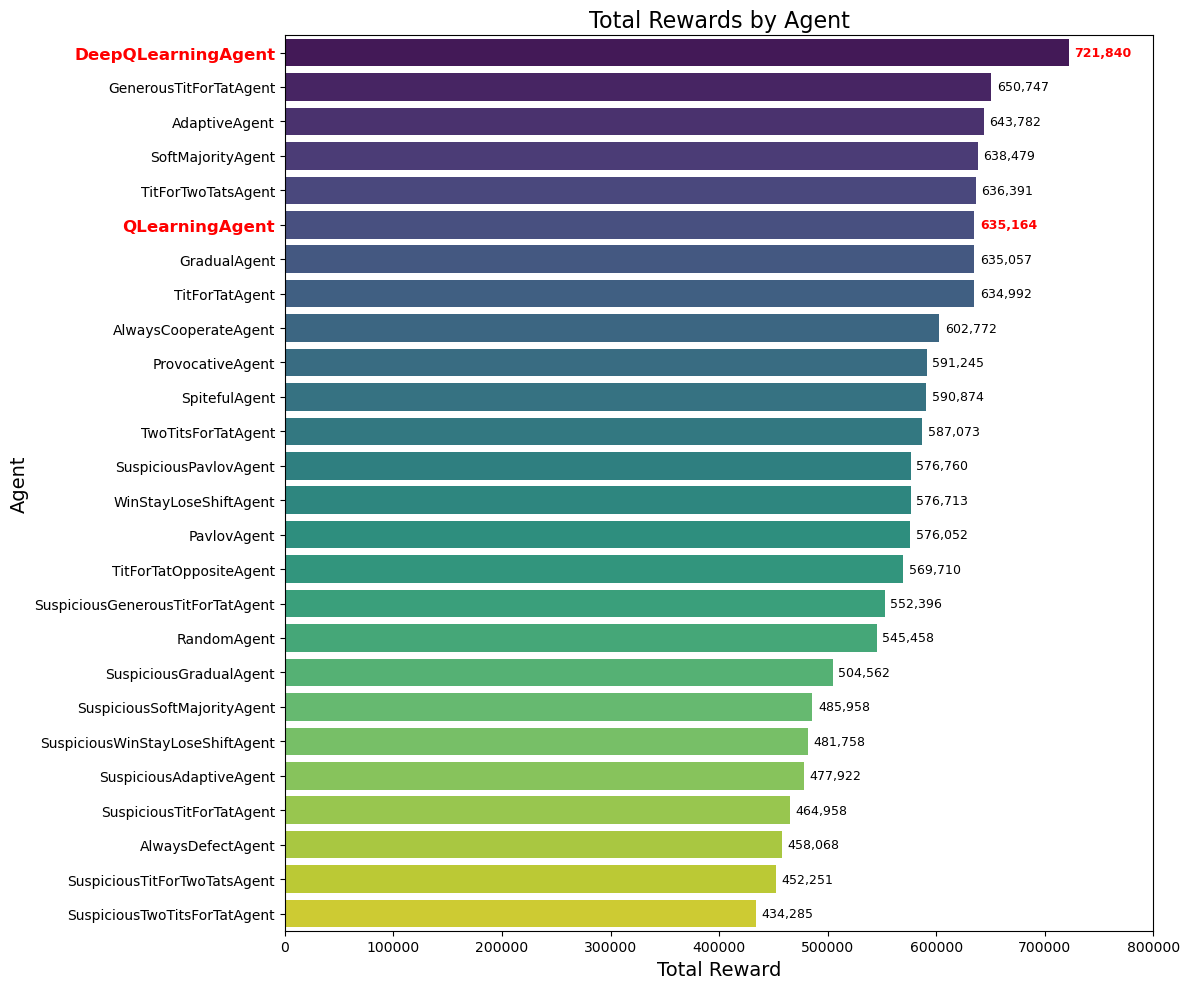
\includegraphics[height=10cm]{../poster/logos/tournament.png}
    \caption{Gesamtbelohnungen der Agenten im Turnier}
    \label{fig:gesamtbelohnungen}
\end{figure}
Bevor die Ergebnisse der RL-Agenten genauer analysiert werden, können einige Beobachtungen zusammengetragen werden:
\begin{itemize}
    \item \textit{Suspicious} Agenten schneiden insgesamt schlechter ab.
    \item Die beste Basis-Strategie ist \textit{GenerousTitForTat}.
    \item Immer zu kooperieren ist besser als immer zu defektieren.
\end{itemize}
Diese Beobachtungen decken sich auch mit den Entdeckungen, die Robert Axelrod in seinem Buch 
\textit{The Evolution of Cooperation}\footcite{axelrod1984cooperation} gemacht hat.

\subsection{QLearning-Ergebnisse}
Aus dem Training ging folgende Q-Tabelle hervor:
\begin{table}[H]
    \centering
    \begin{tabular}{c|c|c}
            & Q-Werte für Kooperation & Q-Werte für Defektion \\
        \hline
        Gegner kooperierte &  52.7929238 & 2.61803697\\
        \hline
        Gegner defektierte &  0.9977664 & 53.59111475 \\
    \end{tabular}
    \caption{Q-Tabelle nach dem Training}
    \label{table:qtableaftertraining}
\end{table}
Da $Q(0, 0) > Q(0, 1) \land Q(1, 0) < Q(1, 1)$ gilt, konvergierte der \textit{QLearningAgent} offentsichtlich in Richtung des
\textit{TitForTatAgent}'s. Dies spiegelt sich auch in den Tunierergebnissen (siehe Abb. \ref{fig:gesamtbelohnungen}) wieder:
Dort reiht sich der QLearning-Agent auch dort ein. Durch unterschiedliche Entscheidungen von Agenten, die auf Wahrscheinlichkeiten 
beruhen (\textit{RandomAgent(), \textit{GenerousTitForTatAgent()}}) gibt es minimale Abweichungen zwischen den Agenten.
Wenn man diese Ergebnisse mit denen der anderen drei Strategien, die der \textit{QLearningAgent()} entwickeln konnte vergleicht,
fällt auf, dass die TitForTat-Strategie langfristig die besten Ergebnisse erzielt. Es gilt:
TitForTatAgent() > AlwaysCooperateAgent() > TitForTatOppositeAgent() > AlwaysDefectAgent().
Die Verteilung von Kooperation und Defektion des \textit{QLearningAgent}'s ist in Abb. \ref{fig:qverteilung} dargestellt:
\begin{figure}[H]
    \centering
    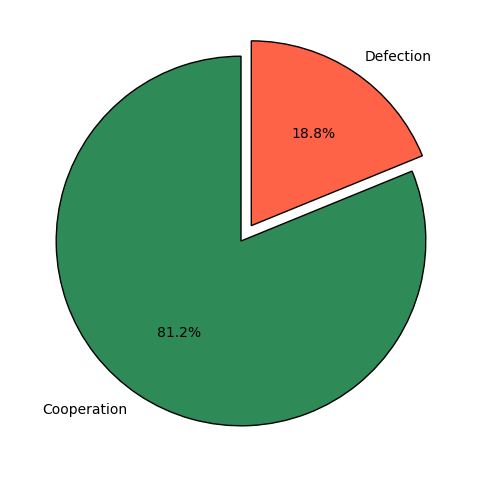
\includegraphics[width=7cm]{../poster/logos/qPie.png}
    \caption{Verteilung von Kooperation und Defektion des \textit{QLearningAgent}'s}
    \label{fig:qverteilung}
\end{figure}

\subsection{Deep QLearning-Ergebnisse}
Der \textit{DeepQLearningAgent} geht als Sieger des Tuniers hervor mit durschnittlich $741597 / 2400 \approx 309$ Belohnungen pro Spiel. 
Die folgende Grafik zeigt die Verteilung von Kooperation und Defektion über alle Spiele im Turnier:
\begin{figure}[H]
    \centering
    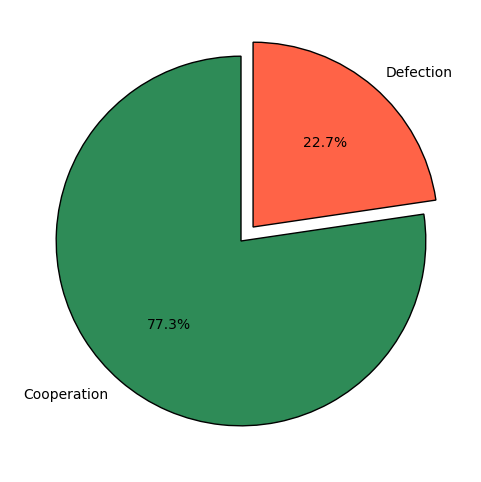
\includegraphics[width=7cm]{../poster/logos/deepqPie.png}
    \caption{Verteilung von Kooperation und Defektion des \textit{DeepQLearningAgent}'s}
    \label{fig:deepqverteilung}
\end{figure}
Damit defektiert der \textit{DeepQLearningAgent} öfter als der \textit{QLearningAgent}, aber auch hier zeigt sich wieder: Es lohnt sich 
häufig zu kooperieren. 

Um besser zu verstehen wie der \textit{DeepQLearningAgent} agiert, kann man sich anschauen, wie er seine Strategie
je nach Gegner anpasst. Gegen die meisten Strategien setzt er auf langfristige Kooperation und defektiert nur sehr selten, es gibt
aber auch einige Ausnahmen:
Gegen den \textit{SoftMajorityAgent()} wäre die beste Strategie abwechselnd zu koopieren und zu defektieren. Der
\textit{DeepQLearningAgent} erkennt dies und defektiert in fast 50\% der Runden. Gegen den \textit{ProvocativeAgent()} defektiert er
fast immer, genauso wie gegen den \textit{TitForTatOppositeAgent()}, was in beiden fällen auch sinnvolle Strategien sind. Gegen den 
\textit{TitForTwoTatsAgent()} defektiert er ebenfalls in ungefähr 50\% der Runden. Teilweise ''verwechselt'' der \textit{DeepQLearningAgent}
seine Gegner und defektiert z.B. nur alle 2 Runden gegen den \textit{AlwaysCooperateAgent()}. Gegen den \textit{AlwaysDefectAgent()}
und den \textit{SpitefulAgent()} hat er jedoch Probleme und kooperiert häufig. 

Insgesamt muss man anerkennen, dass ein ''perfektes'' Ergebnis nicht möglich ist. Im Verhalten des \textit{DeepQLearningAgent} erkennt man ebenfalls,
dass er zuerst ''testet'', gegen welchen Gegner er spielt. Das ist notwenig, um die Strategie anzupassen, führt aber auch zum Verlust von Punkten.
Beim \textit{SpitefulAgent()} z.B. ist es aber schon zu spät, wenn man erkennt, dass dieser der Gegner ist. \\ \\
Durch diese Mischung aus langfristiger Kooperation und Ausnutzen von Schwachstellen in der gegnerischen Strategie ist der 
\textit{DeepQLearningAgent} in der Lage langfristig zu gewinnen und jede andere Strategie zu übertreffen.
    \chapter{Diskussion}
\section{Interpretation der Ergebnisse}
\section{Vergleich mit Erwartungen}
\section{Limitationen}
    \chapter{Fazit}
\section{Zusammenfassung der Ergebnisse}
Zusammenfassend zeigen die Ergebnisse, dass Reinforcement Learning eine effektive Methode ist, um erfolgreiche Strategien für wiederholte 
soziale Dilemmata zu entwickeln. Während der Q-Learning-Agent die beste für ihn mögliche Strategie findet, hebt sich der Deep Q-Learning-Agent 
durch seine anpassungsfähige und opportunistische Spielweise hervor. Dies unterstreicht die Stärke von Deep Learning in strategischen 
Entscheidungsszenarien. Trotz einzelner Schwächen zeigt sich, dass lernfähige Agenten klassische, statische Strategien langfristig übertreffen können.
Die anfängliche Hypothese hat sich also als richtig erwiesen.

\section{Ausblick}
Die Entscheidung für die gewählten RL-Algorithmen ist abschließend als richtig zu bewerten, insbesondere die Anwendung von Deep Q-Learning.

Dennoch gibt es einige Herausforderungen und 
offene Fragen, die in zukünftigen Arbeiten weiter untersucht werden sollten.

Ein interessantes Thema für zukünftige Forschungen könnte die Anwendung von Langzeitgedächtnisstrategien sein, 
wie sie in rekurrenten neuronalen Netzwerken (RNNs) oder Long Short-Term Memory-Netzwerken (LSTMs) zu finden sind. 
Diese könnten es den Agenten ermöglichen, frühere Interaktionen und Muster in den Entscheidungen des Gegners besser zu berücksichtigen 
und ihre Strategie entsprechend anzupassen. Auch der Einfluss von ``Vergessen'' in diesen Netzwerken könnte interessante neue 
Erkenntnisse liefern, da in manchen Situationen das Behalten von Informationen über sehr lange Zeiträume kontraproduktiv sein könnte.

Die Untersuchung alternativer Netzwerk-Architekturen und Hyperparametern ist ein weiteres Feld für zukünftige Arbeiten. 
Dies würde es ermöglichen, das Potenzial der Agenten weiter zu maximieren.

Schließlich ist auch die Frage nach der Erklärbarkeit der Entscheidungen von Deep Q-Learning-Agenten ein spannendes Thema. 
Während diese Agenten in Bezug auf die Performance herausragend sind, bleibt es oft unklar, warum sie bestimmte Entscheidungen treffen. 
In sicherheitskritischen oder ethisch sensiblen Anwendungen könnte es entscheidend sein, diese Entscheidungen nachvollziehbar 
und transparent zu machen. Ansätze wie Explainable AI könnten hier dazu beitragen, die Zugänglichkeit und das 
Vertrauen in die Modelle zu verbessern.

Insgesamt zeigt die Forschung, dass Reinforcement Learning und Deep Learning das Potenzial haben, die Entscheidungsfindung in sozialen Dilemmata zu revolutionieren. Dennoch bleibt noch viel Raum für Verbesserung und Erweiterung, um die Agenten noch robuster und anpassungsfähiger zu machen, insbesondere in realeren Szenarien, in denen Unsicherheit und Komplexität eine größere Rolle spielen.

    
    
	
	
	%Referenzen
    %\bibliographystyle{apalike}
	%\bibliography{bibliography}
	
	%\printglossary[type=\acronymtype]
    %\printglossary
	

    % \cleardoublepage{}
	%\pagebreak
	
	%add your end matter here
% 	\appendix{}

	%\input{C) Back Matter/appendix}
	
	
	
\end{document}